%% This is an example first chapter.  You should put chapter/appendix that you
%% write into a separate file, and add a line \include{yourfilename} to
%% main.tex, where `yourfilename.tex' is the name of the chapter/appendix file.
%% You can process specific files by typing their names in at the 
%% \files=
%% prompt when you run the file main.tex through LaTeX.
\newenvironment{mylisting}
{\begin{list}{}{\setlength{\leftmargin}{1em}}\item\scriptsize\bfseries}
{\end{list}}

\chapter{Overcoming Nondeterminism in Linux services}
This chapter first broadly summarizes the sources of nondeterminism
in Linux services discovered through our experiments (Section \ref{ch3:sources}).
Next, it explains the dynamic instrumentation techniques
we used to simulate deterministic execution in a boot
storm scenario (Section \ref{ch3:simulation}).
Finally, it discusses some of the limitations 
in our approach to deterministic execution (Section \ref{ch3:issues}).

\section{Sources of Nondeterminism} \label{ch3:sources}
In this section, we describe the sources of nondeterminism
that we discovered using the data collection scheme
described in Chapter \ref{ch:boot}.
This study of nondeterminism reveals
subtle interactions between user-mode
applications, commonly used system libraries (e.g. the \texttt{libc} library),
the Linux operating system and the external world.
While our results are derived from analyzing a small
set of complex programs, they include
all sources of application-level nondeterminism that 
have been described in literature. Unlike existing work,
we cover the various interfaces between user-mode programs
and the Linux kernel in considerable detail.

\subsection{Linux Security Features} \label{ch3:security}
\noindent {\bf Address Space Layout Randomization (ASLR)} \newline
Address Space Layout Randomization (ASLR) involves random arrangement of
key memory segments of an executing program. When ASLR is enabled,
the virtual addresses for the base executable, shared libraries, 
the heap, and the stack are different every time the program is run.
ASLR hinders several kinds of security attacks in which attackers have to predict
program addresses in order to redirect execution (e.g. \emph{return-to-libc} attacks). 
As mentioned earlier, two execution traces of even a
simple one-line program in $C$ are almost entirely different
when ASLR is enabled because of differences in
instruction and memory addresses. \newline

\noindent {\bf Canary Values and Stack Protection} \newline
Copying a \emph{canary} -- a dynamically chosen global value -- onto the
stack before each function call can help detect buffer overflow attacks, because 
an attack that overwrites the return address will also overwrite
the copy of the canary. Before a \texttt{ret}, a simple comparison 
of the global (and unchanged) canary
value with the (possibly changed) stack copy can prevent a buffer overflow attack.

In 32-bit Linux distributions, the $C$ runtime library, 
\texttt{libc}, provides a canary value in \texttt{gs:0x14}.
If Stack Smashing Protection (SSP) is enabled on compilation,
\texttt{gcc} generates instructions that use the canary value
in \texttt{gs:0x14} to detect buffer overflow attacks.
Because Pin gets control of the application before \texttt{libc}
initializes \texttt{gs:0x14}, multiple execution traces of a program
will diverge when \texttt{gs:0x14} is initialized and subsequently
read.  The manner in which the canary value in \texttt{gs:0x14} is initialized
depends on the \texttt{libc} version.
If randomization is disabled, \texttt{libc} will store a fixed
terminator canary value in \texttt{gs:0x14}; this does not lead to any nondeterminism.
When randomization is enabled, however,  
some versions of \texttt{libc} store a random word in \texttt{gs:0x14} 
by reading from \texttt{`/dev/urandom'}
or by using the \texttt{AT\_RANDOM} bytes provided by the kernel (see
Section \ref{ch3:rand}). 

\newpage
\noindent {\bf Pointer Encryption} \newline
Many stateless APIs return data pointers to clients 
that the clients are supposed to simply supply as arguments
to subsequent function calls. 
For instance, the \texttt{setjmp} and \texttt{longjmp} functions
can be used to implement a try-catch block in $C$: \texttt{setjmp} uses 
a caller-provided, platform-specific \texttt{jmp\_buf} structure
to store important register state that \texttt{longjmp} later reads to simulate a return from \texttt{setjmp}.
Since the \texttt{jmp\_buf} instance is transparent to clients of \texttt{setjmp}
and \texttt{longjmp}, it is possible that the clients may advertently or inadvertently
overwrite the return address stored in it and simulate a buffer-overflow attack
via \texttt{longjmp}.

Simple encryption schemes can detect mangled data structures.
For instance, in 32-bit Linux, \texttt{libc} provides
a {\em pointer guard}  in \texttt{gs:0x18}. 
The idea behind the pointer guard is the following: 
to encrypt a sensitive address $p$, a program
can compute $s = p$  $\oplus  $ \texttt{gs:0x18}, 
optionally add some bit rotations, and store it in a structure
that gets passed around. Decryption can simply invert any bit rotations, 
and then compute $p = s$ $\oplus  $ \texttt{gs:0x18} back. 
Any blunt writes to the structure from clients will be detected because
decryption will likely not produce a valid pointer. 
Pointer encryption is a useful security feature for some APIs
and is used by some versions of \texttt{libc} to protect addresses stored in \texttt{jmp\_buf}
structures.

This pointer guard has different values
across multiple runs of a program, just like the \texttt{libc} canary
value. Initialization of the \texttt{libc} pointer guard can 
therefore be a source of nondeterminism in program execution. 
In some versions of \texttt{libc}, the value of \texttt{gs:0x18} is the same
as the value of \texttt{gs:0x14} (the canary). In others,
the value of \texttt{gs:0x18} is computed by \texttt{XOR}ing \texttt{gs:0x14} with 
a random word (e.g. the return value of the \texttt{rdtsc} x86 instruction),
or reading other \texttt{AT\_RANDOM} bytes provided by the kernel
 (Section \ref{ch3:rand}).

\subsection{Randomization Schemes} \label{ch3:rand}
As already clear from Section \ref{ch3:security}, 
randomization schemes constitute a major source of nondeterminism 
in programs. Applications generally use pseudorandom number generators (PRNGs)
for randomization and rely on the {\em seeds} to the PRNGs
to be different across multiple program executions 
to generate truly random values. PRNG seeds are typically 
computed from several external sources:

\begin{itemize}

\item {\em The} \texttt{`/dev/urandom'}{\em special file}: Linux allows
running processes to access a random number generator through this
special file. The entropy generated from environmental noise (including
device drivers) is used in some implementations for the kernel random number generator.

\item \texttt{AT\_RANDOM} {\em bytes}: 
Making system calls to open, read and close the
\texttt{`/dev/urandom'} file only for a
few random bytes can be computationally expensive. To
remedy this, some 
recent versions of the Linux kernel supply
a few random bytes to all executing programs
through the \texttt{AT\_RANDOM} auxiliary vector.
ELF auxiliary vectors are pushed on the program
stack below command-line arguments and environmental
variables before a program starts executing.

\item {\em The} \texttt{rdtsc} {\em instruction}:
The \texttt{rdtsc} instruction provides an approximate number of ticks since
the computer was last reset, which is stored in a 64-bit register present
on x86 processors. Computing the difference between two successive
calls to \texttt{rdtsc} can be used for timing, whereas a single
value returned from \texttt{rdtsc} lacks any useful context.  
The instruction has low-overhead, which makes it suitable for generating a random value
instead of reading from \texttt{`/dev/urandom'}. 

\item {\em The current time or process ID}: Many applications simply make a system call
to get the current time or the current process ID, and use the returned value to seed their PRNGs. 

\item {\em Miscellaneous}: There
are several creative ways to seed random number
generators (e.g. read from {\em www.random.org}),
but thankfully we have not observed them
in the Linux services we have analyzed.
\end{itemize}

Thus, true nondeterminism in Linux services is caused
from the external techniques used to seed PRNGs;
if the seeds are different across multiple
executions, PRNGs algorithms propagate this
nondeterminsm much further.

\subsection{Process Identification Layer} \label{ch3:pid}
% pid, signal(pid), /proc/ filesystem layer

In the absence of a deterministic operating system layer, process IDs assigned
to Linux services at boot-time are not predictable.
For instance, a nondeterministic scheduler (Section \ref{ch3:concurrency}) 
could lead to several possible process creation sequences
and process ID assignments.

Given the unpredictability of process IDs,
system calls that directly or indirectly
interact with the process identification layer can cause divergences
in distinct executions of the same program.
For instance, system calls that return a process ID e.g.
\texttt{getpid} (get process ID), \texttt{getppid} (get
parent process ID), \texttt{fork/clone} (create a child process),
\texttt{wait} (wait for a child process to terminate)
can return different values across executions. System calls that take process IDs 
directly as arguments such as \texttt{kill} (send a signal to a specific
process), \texttt{waitpid} (wait for a specific child process to terminate)
can similarly propagate any nondeterminism.
In fact, \texttt{libc} stores a copy of the current process ID in \texttt{gs:0x48},
so reads or writes to this address can cause conflicts.

Apart from system calls, there are other interfaces
between the Linux kernel and executing user-mode programs
where process IDs also show up:

\begin{itemize} 

\item {\em Signals}: If a process registers a signal handler with the \texttt{SA\_SIGINFO}
bit set, then the second argument passed
to the signal handler when a signal occurs is of type \texttt{siginfo\_t*}.
The member \texttt{siginfo\_t.si\_pid} will
be set if another process sent the signal 
to the original process. (Section \ref{ch3:sig}). 

\item {\em Kernel messages}: The Linux kernel will sometimes use process IDs 
to indicate the intended recipients of its messages. 
For instance, \texttt{Netlink} is a socket-like
mechanism for inter process communications (IPC)
between the kernel and user-space processes.
\texttt{Netlink} can be used to pass
networking information between kernel
and user-space, and some of its APIs 
use process IDs to identify communication
end-points. (Section \ref{ch3:netio}). \end{itemize}

\newpage 
Nondeterminism arising from the unpredictability of process IDs can be
further propagated when process IDs are used to seed PRNGs (Section \ref{ch3:rand}),
access the \texttt{`/proc/[pid]'} directory (Section \ref{ch3:procfs}),
and create application-specific files or write to them. (Section \ref{ch3:fileio}). 

\subsection{Time} \label{ch3:time}
Concurrent runs of the same program will typically
execute the same instructions at (slightly) different times.
Clearly, any interactions of a program with timestamps
can cause nondeterminism. For instance:

\begin{itemize}
\item The \texttt{time}, \texttt{gettimeofday} and \texttt{clock\_gettime}
 system calls return the current time.
\item The \texttt{times} or \texttt{getrusage} system calls
return process and CPU time statistics respectively.
\item The \texttt{adjtimex} system call is used 
by clock synchronization programs (e.g. \texttt{ntp}) 
and returns a kernel timestamp indirectly via 
a \texttt{timex} structure.
\item Programs can access the hardware clock
through \texttt{`/dev/rtc'} and read the current time
through the \texttt{RTC\_RD\_TIME} \texttt{ioctl}
operation.
\item Many system calls that specify a timeout
for some action (e.g. \texttt{select}, \texttt{sleep} or \texttt{alarm})
inform the caller of any unused time from the timeout interval if they
return prematurely.
\item The \texttt{stat} family of system calls returns file
  modification timestamps; also, many application files typically contain timestamps;
  network protocols use headers with timestamps as well (Sections \ref{ch3:fileio}
  and \ref{ch3:netio}).
\end{itemize}

Apart from nondeterminism arising
from timestamps, {\em timing} differences
can arise between distinct executions 
because of variable system-call latency 
or unpredictable timing
external events relative
to program execution (Sections \ref{ch3:sig} and \ref{ch3:poll}).

\subsection{File I/O} \label{ch3:fileio}
\noindent {\bf File contents} \newline
If two executions of the same program read different
file contents (e.g. cache files), then
there will naturally be some execution divergence.
However, for concurrently executing Linux services,
differences in file contents typically arise
from process IDs (Section \ref{ch3:pid}) or timestamps (Section \ref{ch3:time})
rather than semantic differences.
If those factors are controlled, file contents rarely differ. \newline

\noindent {\bf File Modification Times} \newline
Apart from minor differences in file contents,
nondeterminism can arise from distinct file 
modification (\texttt{mtime}), access (\texttt{atime}) or status-change (\texttt{ctime})
timestamps.
The \texttt{stat} system call is usually made for almost
every file opened by a program; the timestamps
in the buffer written by the system call invariably
conflict between any two executions. Most of the time,
these timestamps are not read by programs,
so there is little propagation. On occasion, 
however, a program will use these timestamps
to determine which file out of a group is the most recent, 
or whether a file has been updated
and needs to be refreshed. \newline

\noindent {\bf File Size} \newline
When a program wishes to open
a file in append-mode, it uses \texttt{lseek}
with \texttt{SEEK\_END} to move
the file cursor to the end,
before any \texttt{write}s take place.
The return value of \texttt{lseek} is the
updated cursor byte-offset into the file.
Clearly, if the length of a file is different across
multiple exections of a program, then
\texttt{lseek} will return conflicting values.
Many Linux services maintain log files
which can have different lengths due
to conflicts in an earlier execution; \texttt{lseek}
further propagates them. To overcome
such nondeterminism, older log files
must be identical at the beginning 
of program execution and other
factors that cause nondeterminism
must be controlled. 

\newpage
Ultimately, however, if two input or configuration files
are semantically different between
different executions of a program, then 
execution will inevitably diverge. 

\subsection{Network I/O} \label{ch3:netio}
\noindent {\bf Network Configuration Files} \newline
The \texttt{libc} network initialization
code loads several configuration files
into memory (e.g. \texttt{`/etc/resolv.conf'}). 
Differences in the content, timestamps or lengths
of such configuration files can clearly cause nondeterminism.
Background daemons (e.g. \texttt{dhclient} for \texttt{`/etc/resolv.conf'}) 
usually update these files periodically in the background.
Calls to \texttt{libc} functions such as \texttt{getaddrinfo} use \texttt{stat} 
to determine if relevant configuration files (e.g. \texttt{`/etc/gai.conf'})
have been modified since they were last read. 
In our experiments, typically the file modification timestamps 
-- and not the actual contents -- of these configuration files vary between different executions,
because identical VMs have the same network setup. \newline

\noindent {\bf DNS Resolution} \newline
In our experiments, IP addresses are resolved identically by concurrently executing services. 
However, if DNS-based load-balancing schemes are used, the same 
servers can appear to have different IP addresses. \newline

\noindent {\bf Socket \texttt{read}s} \newline
Bytes read from sockets can differ between
executions for a variety
of reasons. For instance, different timestamps in 
protocol headers, or different requests/responses 
from the external world would be reflected in
conflicting socket \texttt{read}s.
By studying application behavior, it is possible
to distinguish between 
these different scenarios and
identify the seriousness
of any differences from socket reads.

In our experiments, we have only observed nondeterminism
in \texttt{read}s from \texttt{Netlink} sockets.
As mentioned in Section \ref{ch3:pid},
\texttt{Netlink} sockets provide a 
mechanism for inter-process communications (IPC)
between the kernel and user-space processes.
This mechanism can be used to pass
networking information between kernel
and user space. \texttt{Netlink} sockets
use process IDs to identify
communication endpoints, which can
differ between executions (Section \ref{ch3:pid}).
Some implementations of \texttt{libc} use
the current time as sequence
number for \texttt{Netlink} packets (Section \ref{ch3:time}).
Also, a
socket of the \texttt{NETLINK\_ROUTE}
family receives routing and link updates
from the kernel. \texttt{libc} uses \texttt{RTM\_NEWLINK}
messages to discover the link interfaces 
in the computer. When a new interface
is discovered or reported, the kernel also supplies
interface statistics to \texttt{libc},
such as packets/bytes sent, dropped or
received. These statistics will obviously be different
across different executions.  \newline

\noindent {\bf Ephemeral Ports} \newline
A TCP/IPv4 connection consists of two end-points;
each end-point consists of an IP address and a port
number. An established client-server connection 
can be thought of as the
4-tuple (server\_IP, server\_port, client\_IP, client\_port).
Usually three of these four are readily known:
a client must use its own IP, and
the pair (server\_IP, server\_port) is fixed. What is not
immediately evident is that the client-side of 
the connection uses a port number.
Unless a client program explicitly
requests a specific port number,
the port number used is for an {\em ephemeral port}.
Ephemeral ports are temporary ports
assigned from a dedicated range by the machine IP stack,
When a connection
terminates, an ephemeral port can be recycled.
Since the underlying operating system
is not deterministic, ephemeral
port numbers used by Linux services
tend to be different across multiple 
runs. 

\subsection{Scalable I/O Schemes} \label{ch3:poll}
\noindent {\bf Polling Engines} \newline
Complex programs like Linux services have
many file descriptors open at a given time.
Apart from regular files, these file descriptors could correspond to:

\begin{itemize}

\item {\em Pipes}: Pipes are used for
  one-way interprocess communication (IPC).
  Many Linux services spawn child processes;
  these child processes communicate
  with the main process (e.g. for status
  updates) through these pipes.

\item A {\em listener socket}:
  If the program is a server,
  this is the socket that accepts incoming connections.

\item {\em Client-handler sockets}:
  If this program is a server, 
  new requests from already connected clients would arrive through
  such sockets.

\item {\em Outgoing sockets}:
  If the program is a client for other servers,
  it would use these sockets to send requests 
  to them.
\end{itemize}

The classic paradigm for implementing server
programs is {\em one thread or process per client}
because I/O operations are traditionally blocking
in nature. This approach scales poorly as the number
of clients -- or equivalently, the number of open file descriptors -- increases. 
As an alternative, event-based I/O is increasingly used 
by applications with many open file descriptors.
In event-based I/O, the event-thread
specifies a set of file descriptors it cares about,
and then waits for ``readiness'' notifications 
from the operating system on any of
these file descriptors by using a
system call such as \texttt{epoll}, \texttt{poll},
\texttt{select} or \texttt{kqueue}. 
For instance, a client socket would be ready 
for reading if new data was received from a client,
and an outgoing socket would be ready for 
writing if an output buffer was flushed out or if the 
connection request was accepted.
The event-thread invokes an I/O
handler on received event, 
and then repeats the loop to process the next
set of events.
This approach is often used for design simplicity because it
reduces the threads or processes needed by an application; 
recent kernel implementations (e.g. \texttt{epoll}) are also
efficient because they return the set of file descriptors that are ``ready'' for I/O,
preventing the need for the application to iterate through all its open
file descriptors. 

Event-based I/O can be a source
of nondeterminism in programs because the
timing of I/O events with respect to each other
can be different across multiple executions.
Even if I/O events are received in the same order,
the same amount of data may not be available
from ``ready'' file descriptors. Furthermore, when a timeout
interval is specified by the application for polling file descriptors,
\texttt{select} may be completed or interrupted
prematurely. In that case, \texttt{select} returns
the remaining time interval, which can     
differ between executions (Section \ref{ch3:time}).

\noindent {\bf Asynchronous I/O Systems} \newline
Asynchronous I/O APIs (e.g. the Kernel Asynchronous I/O interface
in some Linux distributions) allow even a single application
thread to overlap I/O operations with other processing
tasks. A thread can request an I/O operation (e.g. \texttt{aio\_read}),
and later query the OS or be notified by it that the I/O operation
has been completed (e.g. \texttt{aio\_return}). While such APIs are in limited
usage, they would create nondeterminism because of the
variable absolute and relative timing of I/O events.

\subsection{Signals}\label{ch3:sig}
A signal is an event generated by Linux
in response to some condition, which may cause
a process to take an action in response.
Signals can be generated by error conditions
(e.g. memory segment violations), 
terminal interrupts (e.g. from the shell), 
inter-process communication (e.g. parent 
sends \texttt{kill} to child process),
or scheduled \texttt{alarm}s. 
Processes register handlers (or function callbacks) for specific signals
of interest, in order to respond to them.

Signals are clearly external to
instructions executed by a single process,
as such, they create nondeterminism 
much the same way as asynchronous I/O.
Signals can be delivered to multiple executions
of the same program in different order.
Even if signals are received in the
same order between different executions,
they can be received at different times
into the execution of a program.

\subsection{Concurrency} \label{ch3:concurrency}
Multiple possible instruction interleavings of 
threads within a single program, 
or of different processes within 
a single operating system are
undoubtedly significant sources
of nondeterminism.
Nondeterminism due to
multi-threading has been extensively
documented, and can cause
significant control flow differences
across executions.

Nondeterminism in the system
scheduler is external to 
program execution, and manifests itself
in different timing or ordering
inter-process communications (e.g.
through pipes, signals, or 
values written to file system logs).

\subsection{{\em Procfs}: The `/proc/' directory}\label{ch3:procfs}
Instead of relying on system-calls, user-space programs
can access kernel data much more easily using {\em procfs}, a hierarchical 
directory mounted at \texttt{`/proc/'}.
Procfs is an interface
to kernel data and system information
that would otherwise be available
via system calls (if at all);
thus, many of the sources of nondeterminsm
already described can be propagated
through it.

For instance, \texttt{`/proc/uptime'} contains time statistics about how
long the system has been running;
\texttt{`/proc/meminfo'} contains statistics about kernel memory management;
\texttt{`/proc/net/'} contains network statistics and IP addresses for interfaces;
\texttt{`/proc/diskstats/'} contains statistcs about any attached disks.
These files will differ across multiple executions
of a program because of nondeterminism in the underlying operating system. 

Apart from accessing system-wide information, a process can access 
information about its open file descriptors through
\texttt{`/proc/[PID]/fdinfo'} (e.g. cursor offsets and status).
Similarly, \texttt{`/proc/[PID]/status'} contains
process-specific and highly unpredictable statistics,
e.g. number of involuntary context switches,
memory usage, and parent process ID.
Performing a \texttt{stat} on files in \texttt{`/proc/[PID]/'}
will reveal process creation time.

\subsection{Architecture Specific Instructions}
Architecture specific instructions such as \texttt{rdtsc}
and \texttt{cpuid} can return different
results across program executions. As mentioned before
(Section \ref{ch3:rand}), the \texttt{rdtsc} instruction provides an approximate number of ticks since
the computer was last reset, which
will differ across executions. The \texttt{cpuid} instruction
returns information about the process and the underlying 
hardware, and its results can vary across different
executions as well.

\section{Simulating Determinism} \label{ch3:simulation}
Figure \ref{ch3:simulation}.

\begin{figure}[h]
  \center
  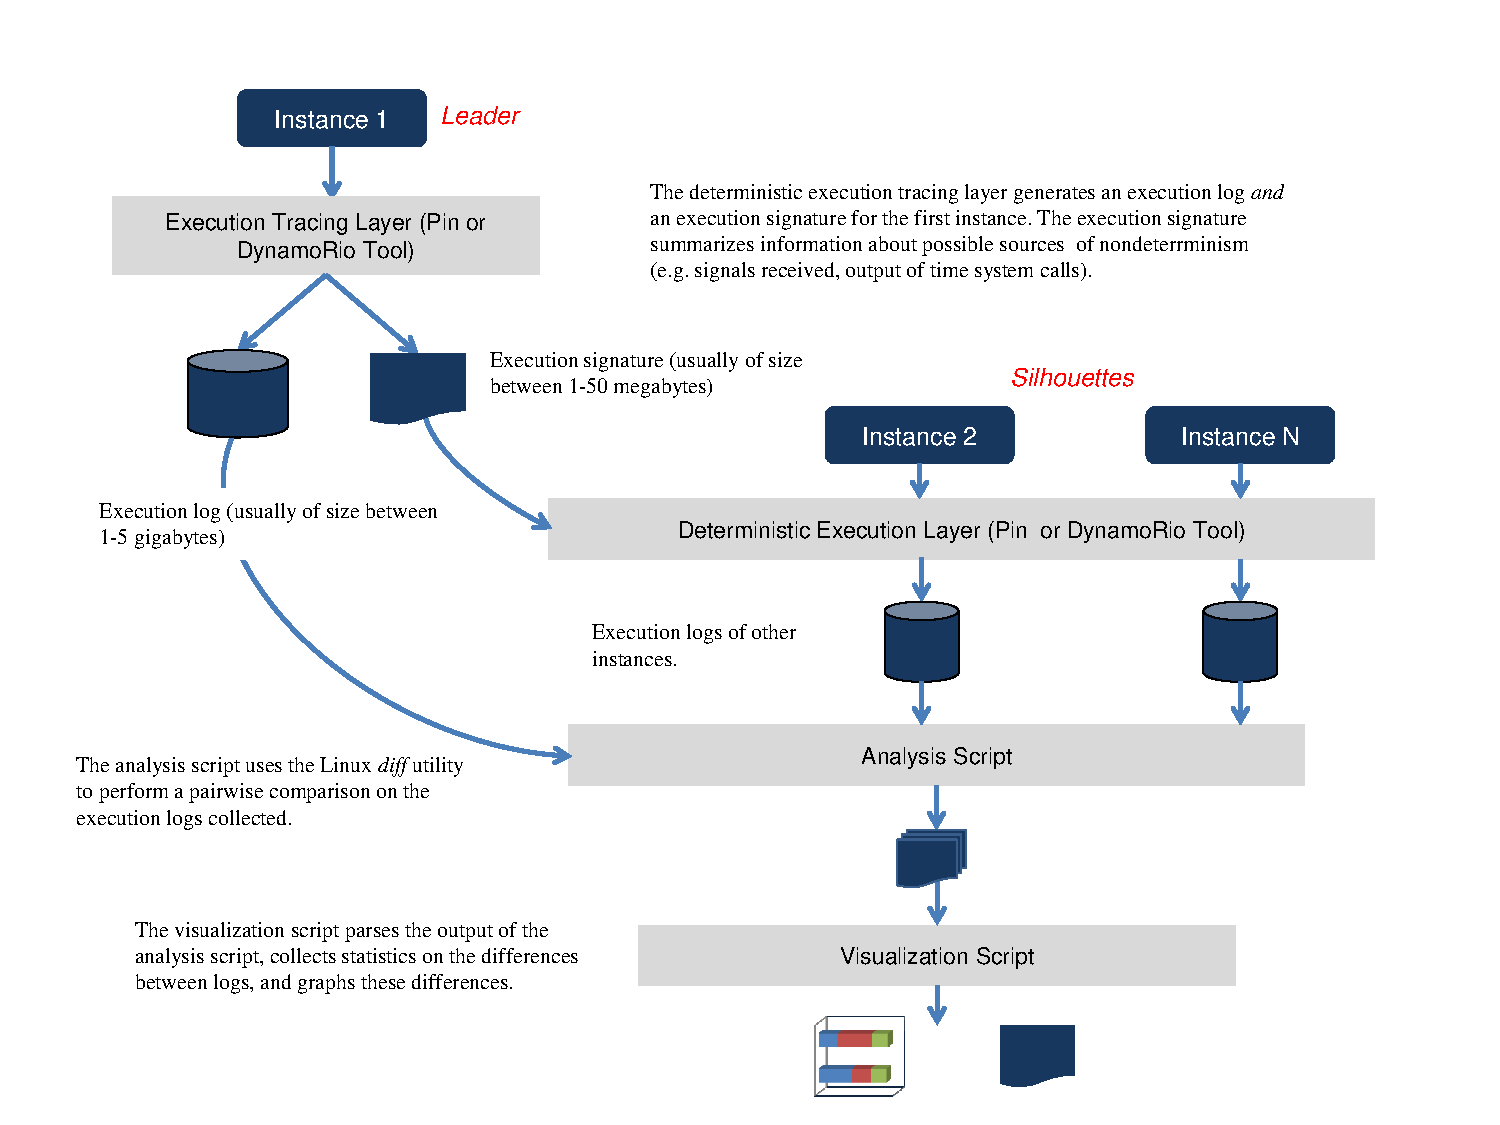
\includegraphics[scale=0.7, trim=1cm 1cm 1cm 1cm]
                  {simulation.pdf}
  \caption[Simulation of Deterministic Execution of Bootstorm scenario]%
  {Simulation of Deterministic Execution of Bootstorm scenario.}
  \label{ch3:simulation}
\end{figure}

Existing record-and-replay systems sometimes overcome ASLR by
forcing the operating system to use the same address space layout across
different runs. A slightly more complicated approach would involve
using base/offset computations to translate equivalent 
addresses between two different executions. 
We simply disabled ASLR for our experiments using the following command:
\texttt {sudo kernel.randomize\_va\_space=0}.



Dynamic instrumentation can be used to force canary values
to agree across distinct executions of the same program:
instructions that initialize \texttt{gs:0x14} can be
modified or replaced, or the \texttt{AT\_RANDOM} bytes provided by the kernel can be
modified before they are read by the application, or reads from \texttt{`/dev/urandom'} can be 
intercepted.

 In any case, the value of the pointer
guard can be made to agree across different instances
of the same program via dynamic instrumentation: 
the instructions that initialize \texttt{gs:0x18} can
be modified or replaced, or the \texttt{rdtsc} instruction
can be intercepted and emulated, or the  \texttt{AT\_RANDOM} bytes provided by the kernel can be
replaced before they are ever read.

To overcome nondeterminism resulting from randomization, 
we need to intercept the standard techniques
used by programs to seed PRNGs.
Dynamic instrumentation can be used to 
intercept reads from \texttt{`/dev/urandom'}
and emulate \texttt{rdtsc} instructions.
Nondeterminism from process IDs
can be controlled by virtualizing the process ID
layer (Section \ref{ch3:pid}), and nondeterminism
from time can be controlled by intercepting
time-related system calls and forcing
agreement between concurrently executing 
instances (Section \ref{ch3:time}).

\begin{figure}[h]
  \center
  
\includegraphics[trim=0cm 0cm 0cm 0cm, scale=0.75]{none.jpg}
  \caption[Virtualizing the process ID layer using Pin]% 
  {We intercept all system calls and communications
  between the Linux user and kernel space; we
  translate between real and virtual process IDs
  to trick the kernel and the user-space programs.}
  \label{ch3:pidfig}
\end{figure} 

Figure \ref{ch3:pidfig} shows how we can use dynamic instrumentation
techniques to virtualize and determinize the process ID layer in Linux.
Using these techniques, we were able to avoid modifying
the Linux operating system and existing programs
altogether.

To overcome nondeterminism from time-related system calls,
we can use dynamic instrumentation to force agreement between 
any timestamps returned across concurrent
executions (taking care to preserve monotonicity).
This creates the illusion that multiple executions
are occuring precisely at the same time. When timestamps
returned from system calls are only compared, they
can be replaced with deterministic ordinal values that 
perserve the comparison (e.g 0 or 1). 

In order to overcome nondeterminism caused
by signal delivery, we reorder signals 
across multiple executions using
dynamic instrumentation.
We also ensure that they are delivered 
at precisely the same instructions
across different executions.


Usually, simply
replacing the time values with fixed ordinal values
that preserve the ordering of timestamps is sufficient
to control such nondeterminism.

% file semantic differences cause nondeterminism inevitably
However,
the approaches mentioned in this chapter
are typically sufficient to ensure that
file contents rarely differ in Linux services,
if at all.

%network config files
Contents rarely differ, so the strategies described in Section \ref{ch3:fileio} 
to overcome \texttt{stat} are sufficient to ensure deterministic execution. 

%DNS 
In these rare cases, dynamic instrumentation can be used
to enforce agreement between different executions.

% sockets
If the contents read from sockets
vary across different executions, dynamic instrumentation can be used to 
intercept Linux socket calls
and modify their side-effects to be identical. If
many concurrent executions are reading data from the
same network source, this simply simulates the possibility that all instances
see the same results as the first instance. 
While these semantics are sufficient for most Linux services,
we have not needed to use them: in our experiments,

we have only observed nondeterminism
By studying applications, it is possible
to distinguish between 
these different scenarios, and
identify the seriousness
of any differences from socket reads.

%NETLINK_IFLA_STATS
However,
we can easily use dynamic instrumentation
to intercept \texttt{Netlink} communications
and force these statistics to be
identical.

We mask this nondeterminism 
using dynamic instrumentation by
changing the \texttt{bind} or \texttt{connect} 
system call arguments to explicitly request ports
in the ephemeral range rather than letting the kernel 
assign them; alternatively,
we can also virtualize ephemeral ports
similar to how we virtualize process IDs.

To handle nondeterminism caused by the relative
timing or the amount of data available 
in event-based polling engines, we 
can use dynamic instrumentation to intercept
the corresponding system calls, and
selectively deliver I/O events to order them
identically across executions. 
In our experiments, this approach has been sufficient to 
achieve deterministic execution.

Nondeterminism due to multi-threading
has been extensively documented; there
is a large body of work that
attempts to overcome such nondeterminism
by using deterministic logical clocks
or record-and-replay approaches. 
For our experiments, we did not attempt to enforce
a total order on the instructions executed in multi-threaded
programs and just measured nondeterminism inside each
thread individually. To
overcome nondeterminism caused
by multi-threading, we could incorporate
deterministic logical clocks 
into our design.


Using the schemes described
in Sections \ref{ch3:sig} and 
\ref{ch3:poll}. Existing
work on deterministic
operating systems can
be extended to overcome these issues
in a more systematic manner.

%AIO
Again, dynamic instrumentation techniques that 
reorder such events would be needed.


The solution is to use dynamic instrumentation
to intercept and modify reads 
from procfs.

\section{Limitations of Deterministic Execution} \label{ch3:issues}
% security: canary aslr etc
% performance & correctness: randomization, ntp (time skew), time monotonic,
% IO aggregation. (acquire lock). 
\section {Summary}
